% Offizielle Beispieldatei für beamer-Vorlage aus tubslatex Version 0.3beta2
\documentclass[fleqn,11pt,aspectratio=43]{beamer}

\usepackage[ngerman]{babel}
\usepackage[utf8x]{inputenc}
\usepackage[absolute,overlay]{textpos}
\usepackage{graphicx}
\usetheme[%
 %nexus,%        Nexus Fonts benutzen
  %lnum,%         Versalziffern verwenden
  %cmyk,%<rgbprint>,          Auswahl des Farbmodells
  blue,%<orange/green/violet> Auswahl des Sekundärfarbklangs
  dark,%<light,medium>        Auswahl der Helligkeit
  %colorhead,%    Farbig hinterlegte Kopfleiste
  %colorfoot,%    Farbig hinterlegt Fußleiste auf Titelseite
  colorblocks,%   Blöcke Farbig hinterlegen
  %nopagenum,%    Keine Seitennumer in Fußzeile
  %nodate,%       Kein Datum in Fußleiste
  tocinheader,%   Inhaltsverzeichnis in Kopfleiste
  %tinytocinheader,% kleines Kopfleisten-Inhaltsverzeichnis
  %widetoc,%      breites Kopfleisten-Inhaltsverzeichnis
  %narrowtoc,%    schmales Kopfleisten-Inhaltsverzeichnis
  %nosubsectionsinheader,%  Keine subsections im Kopfleisten-Inhaltsverzeichnis
  %nologoinfoot,% Kein Logo im Fußbereich darstellen
  ]{tubs}

% Titelseite
\title{BibTeX2HTML}
\subtitle{HTML5-Visualisierung von BibTeX-Einträgen mit Hilfe einer DSL}
\author{Marcus Stelke, Sven Frank, Frieder Berthold und Alexander Knüppel}
% Titelgrafik, automatisch beschnitten, Weitere Optionen: <scaled/cropx/cropy>
% \titlegraphic[cropped]{\includegraphics{infozentrum.jpg}}
\titlegraphic[scaled]{
\includegraphics{titlepicture.jpg}}

% Logo, dass auf Titelseiten oben rechts und auf Inthaltsseiten unten rechts
% dargestellt wird. Es wird jeweils automatisch skliert
%\logo{\includegraphics{dummy_institut.pdf}}
\logo{Institut für Softwaretechnik\\und Fahrzeuginformatik}

\begin{document}

\begin{frame}[plain]
\titlepage
\end{frame}

%\begin{frame}{Inhalt}
%\tableofcontents
%\end{frame}

{
\setbeamerfont{frametitle}{size=\fontsize{13}{5}}
\begin{frame}{Projektziel - HTML5-Visualisierung von BibTeX-Dateien\strut}
\begin{textblock*}{3cm}(9cm,1.5cm) % {block width} (coords)

\includegraphics[width=3cm]{../logo.png}
\end{textblock*}
\textbf{Modellierung mit Xtext}
\begin{itemize}
\item Sprache für das BibTeX-Format
\item Sprache zur Konfiguration der Visualisierung 
\begin{itemize}
\item Sortierung
\item Benutzerspezifische Gestaltung (Farbe, Schrifttyp etc.)
\item Ausgabe einer Quellenmakierung (?)
\end{itemize}
\item Validierung von Constraints
\end{itemize}

\textbf{Transformation }
\begin{itemize}
\item T2M-Transformation durch Xtext (Ecore-Modelle für beide DSLs)
\item M2T-Transformation durch Xtend (integrierte Template-Engine)
\end{itemize}

\textbf{Ausgabe}
\begin{itemize}
\item Valides HTML5-Dokument mit Einträgen aus angegebenen BibTeX-Dateien inklusive CSS
\end{itemize} 
\end{frame}
}

\begin{frame}{Workflow}
\begin{figure}
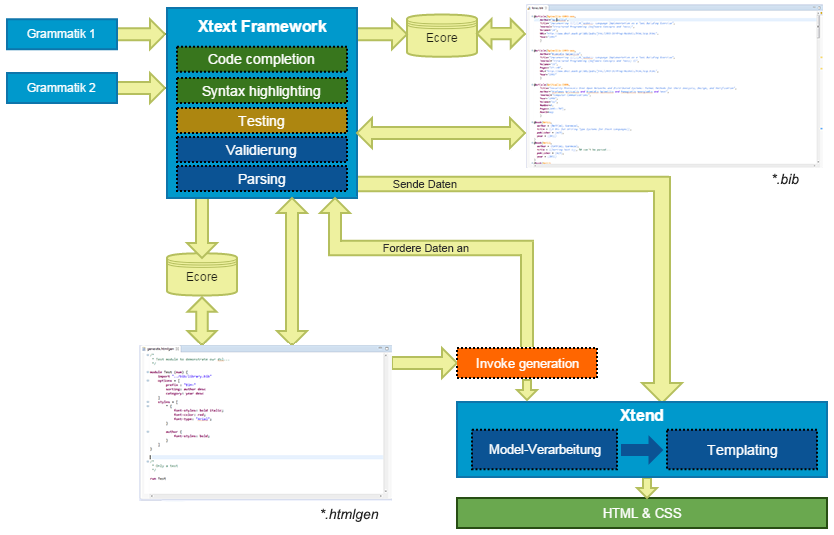
\includegraphics[scale=0.3]{../xtext_workflow.png} 
\caption{Workflow}
\end{figure}
\end{frame}

\begin{frame}{BibTeX-Dateiformat}
\begin{itemize}
\item '@' + Publikations-Typ
\item Schlüsselwort
\item Notwendige und optionale Tags
\end{itemize}
\begin{figure}
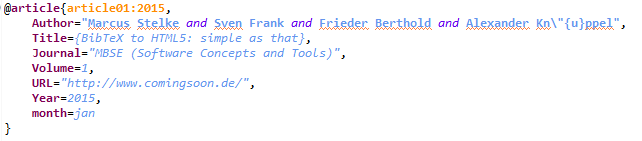
\includegraphics[scale=0.6]{../bibtex_format1.png} 
\end{figure}
\end{frame}

\begin{frame}{Ecore-Metamodell: BibTeX}
\begin{figure}
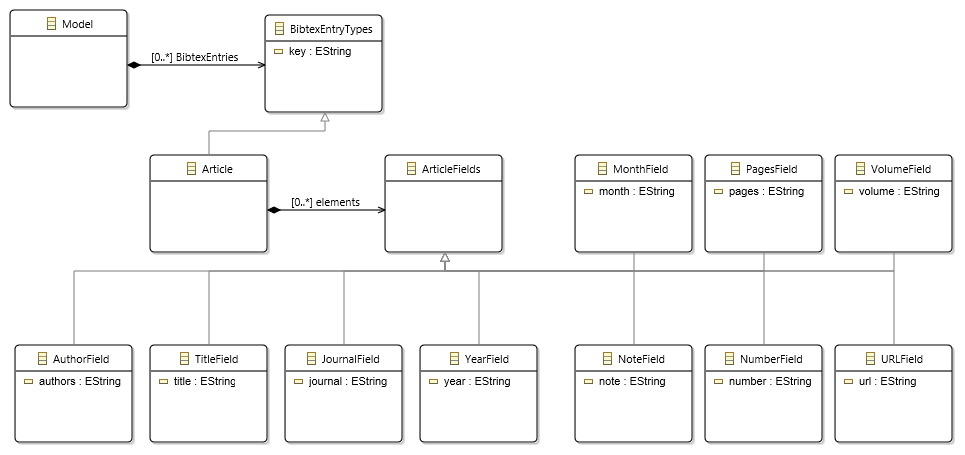
\includegraphics[scale=0.28]{../bibtex_ecore.png} 
\caption{BibTeX: Metamodell}
\end{figure}  
\end{frame}

\begin{frame}{Validierung mit Xtext}
\textbf{Validierung der BibTeX-Einträge}
\begin{itemize}
\item Notwendige Felder \textbf{müssen} genau einmal vorhanden sein
\item Optionale Felder \textbf{dürfen} genau einmal vorhanden sein
\item Unbekannte Felder werden ignoriert
\item BibTeX-Keys einzigartig
\end{itemize}

\textbf{Feldspezifische Validierung (Ausschnitt)}
\begin{itemize}
\item \textit{AuthorsField}
\begin{itemize}
\item mehrere Autoren durch 'and' getrennt
\end{itemize}
\item \textit{PageField}
\begin{itemize}
\item Positive Zahl größer 0
\end{itemize}
\item ...
\end{itemize}
\end{frame}

\begin{frame}{Beispiel 'Unknown field warning'}
In Klasse \textbf{\it BibTeXValidator}:
\begin{figure}
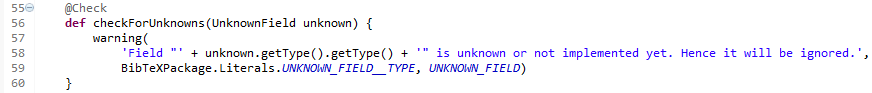
\includegraphics[scale=0.5]{../validation_fragment.png} 
\end{figure} 

Im Editor der Eclipse-Instanz: 
\begin{figure}
\includegraphics<1>[scale=0.5]{../instance_unknownfield1.png} 
\includegraphics<2>[scale=0.5]{../instance_unknownfield2.png} 
\end{figure} 

\end{frame}

\begin{frame}{Ecore-Metamodell: HTML-Generator}
\begin{figure}
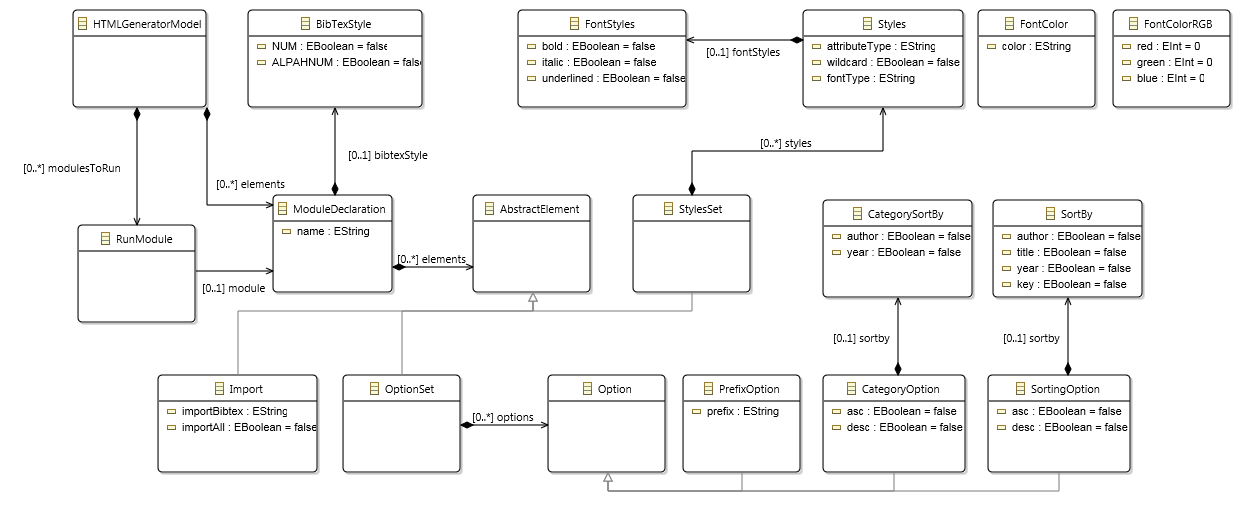
\includegraphics[scale=0.25]{../htmlgen_ecore.png} 
\caption{HTML Generator: Metamodell}
\end{figure}   
\end{frame}

\begin{frame}{Beispiel einer Generator-Datei}
\begin{columns}[t] 
\column{.5\textwidth}
\begin{itemize}
\item Unterteilung in Module
\item Importieren von *.bib-Dateien
\item Diverse Optionen 
\item Unterschiedliche Gestaltung einzelner Felder
\end{itemize}
\column{.5\textwidth}
\begin{figure}
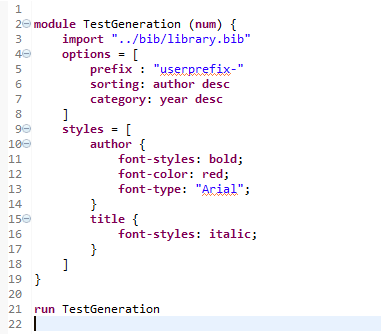
\includegraphics[scale=0.6]{../ExampleHTMLGEN.png} 
%\caption{*.htmlgen}
\end{figure}
\end{columns}
   
\end{frame}

\begin{frame}{Demo}
\centering
\Huge
\textbf{Live-Demo :-)}
\end{frame}

\begin{frame}{Lessons Learned}
\begin{textblock*}{3cm}(9cm,6cm) % {block width} (coords)

\includegraphics[width=3cm]{../logo.png}
\end{textblock*}
\textbf{Allgemein zu Xtext}
\begin{itemize}
\item Gute Trennung der einzelnen Aufgabenbereiche (Grammatik, Validierung, Generierung)
\item Einfach zu benutzen, schwer zu meistern!
\item Ressourcen oftmals unbrauchbar
\end{itemize}

\textbf{Grammatik}
\begin{itemize}
\item Ähnlichkeit mit EBNF
\item Mehrdeutigkeiten oftmals schwer aufzulösen
\end{itemize}

\textbf{Validierung}
\begin{itemize}
\item Verortung von Fehlermeldungen schwierig
\end{itemize}

\textbf{Xtend}
\begin{itemize}
\item Mächtige Spracherweiterung
\end{itemize}

\end{frame}

\end{document}
